% Exact normalized coordinates u=+/-1/2,v=+/-sqrt(3)/2.
\begin{tikzpicture}[x=2.05cm,y=2.05cm,>=stealth,font=\small]
\draw[->,gray] (-1.4,0)--(1.5,0) node[right] {$u=x/a_E$};
\draw[->,gray] (0,-1.15)--(0,1.3) node[above] {$v=y/b_E$};
\draw[blue!70!black,thick] (0,0) circle (1);
\draw[orange!80!black,dashed,thick] (-.5,-1.05)--(-.5,1.05) (.5,-1.05)--(.5,1.05);
\foreach \s in {-1,1} {\foreach \t in {-1,1}
 {\fill[red!75!black] ({\s/2},{\t*sqrt(3)/2}) circle (2.3pt);}}
\node[below left] at (-.5,0) {$-\tfrac12$};
\node[below right] at (.5,0) {$\tfrac12$};
\node[above right] at (.5,{sqrt(3)/2}) {$(\tfrac12,\tfrac{\sqrt3}2)$};
\node at (0,-1.5) {$a_H/c=1/2:\quad u=\pm1/2$};
\end{tikzpicture}
